\section{Auswertung}
\label{sec:Auswertung}
\subsection{Charakteristik des Geiger-Müller-Zählrohrs}

Es wird eine Thallium-Quelle verwendet. \\
Bei Aufnahme der Messwerte für die Charakteristik des Zählrohres wird 
die anliegende Spannung in $10\mathrm{V-Schritten}$ erhöht und bei einer Integrationszeit
von $120$s gemessen.\\
Ungewöhnlich weit abweichende Werte wurden in der Auswertung nicht berücksichtigt. In \autoref{tab:charak} 
sind die einbezogenen Messwerte zu finden. Der gesamte Satz an Messwerten ist in 
\autoref{sec:anhang} aufgelistet.\\

\begin{table}
  \centering
  \caption{Die ausgewerteten Messwerte.}
  \begin{tabular}{ccc}
    \hline
    {$U  \mathbin{/} \unit{\volt}$} &
    {$N \mathbin{/} \mathbin{Imp}$} &
    {$I \mathbin{/} \unit{\micro\ampere}$} \\
    \hline
    330  &  12435  $\pm$ 111   &  0,1   \\
    340  &  13454  $\pm$ 116   &  0,1   \\
    350  &  13651  $\pm$ 117   &  0,1   \\
    360  &  13660  $\pm$ 117   &  0,1   \\
    370  &  13778  $\pm$ 117   &  0,1   \\
    380  &  13770  $\pm$ 117   &  0,1   \\
    390  &  13738  $\pm$ 117   &  0,15  \\
    400  &  14003  $\pm$ 118   &  0,15  \\
    410  &  14192  $\pm$ 119   &  0,18  \\
    420  &  13730  $\pm$ 117   &  0,2   \\
    430  &  14211  $\pm$ 119   &  0,21  \\
    440  &  13861  $\pm$ 118   &  0,21  \\
    480  &  14391  $\pm$ 120   &  0,3   \\
    490  &  14047  $\pm$ 119   &  0,3   \\
    500  &  14092  $\pm$ 119   &  0,3   \\
    510  &  14164  $\pm$ 119   &  0,3   \\
    520  &  14296  $\pm$ 120   &  0,3   \\
    590  &  14337  $\pm$ 120   &  0,4   \\
    600  &  14202  $\pm$ 119   &  0,4   \\
    610  &  14087  $\pm$ 119   &  0,45  \\
    620  &  14180  $\pm$ 119   &  0,45  \\
    630  &  14290  $\pm$ 120   &  0,47  \\
    640  &  14130  $\pm$ 119   &  0,48  \\
    650  &  14466  $\pm$ 120   &  0,5   \\
    660  &  14052  $\pm$ 119   &  0,5   \\
    670  &  14170  $\pm$ 119   &  0,5   \\
    680  &  14589  $\pm$ 121   &  0,52  \\
    690  &  14653  $\pm$ 121   &  0,6   \\
    700  &  14715  $\pm$ 121   &  0,6   \\
    \hline
  \end{tabular}
  \label{tab:charak}
\end{table}

Die Zählraten entsprechen einer Poisson-Verteilung, sodass sich ihr Fehler aus 
\begin{equation*}
  \Delta N = \sqrt{N}
\end{equation*}
ergibt.\\
Die Charakteristik ist in \autoref{fig:charakteristik} graphisch dargestellt.
Der Plateaubereich umfasst das Intervall von 410 V bis 670 V.\\
Die lineare Regression wird mithilfe von Python ([2], [3]) durchgeführt und ergibt
für die Ausgleichsgerade der Parameter $b = (13762 \pm 250)  \: \mathrm{Imp}$ für den y-Achsenabschnitt.
Als Geradengleichung, an die gefitted wird, wird 
\begin{equation*}
  y = mx + b
\end{equation*}
gewählt.\\
Die prozentuale Steigung $m_{\%} = (0,73 \pm 0,45) \mathrm{\frac{\%}{100 V}}$ ergibt sich aus 
\begin{equation*}
  m_{\%} = 100\% \cdot ( \frac{N_{\mathrm{600V}}}{N_{\mathrm{500V}}} - 1 ) ,
\end{equation*}
deren Fehler mit
\begin{equation*}
  \Delta m_{\%} = \frac{100\%}{N_{\mathrm{500V}}} \sqrt{ \frac{N_{\mathrm{600V}}}{N_{\mathrm{500V}}}^2 (\Delta N_{500})^2 +  (\Delta N_{600})^2}
\end{equation*}
berechnet wird.

\begin{figure}[H]
  \centering
  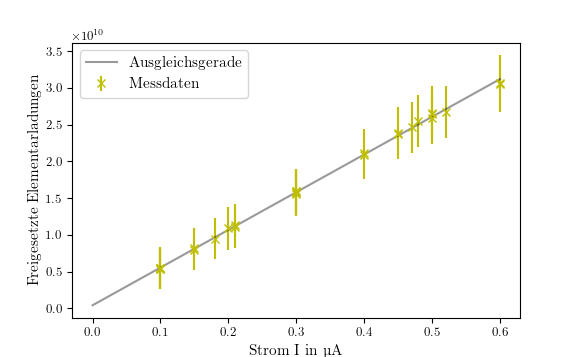
\includegraphics{content/hobelneu.png}
  \caption{Die Charakteristik des Geiger-Müller-Zählrohrs.}
  \label{fig:charakteristik}
\end{figure}


\subsection{Bestimmung der Nachentladungs- und Totzeit}
\subsubsection{Mit Oszilloskop}
Aus dem aufgenommenen Oszillogramm \autoref{fig:totzeit} kann eine Totzeit von 
$T_1 = 130 \mu$s abgelesen werden.\\
\begin{figure}[H]
  \centering
  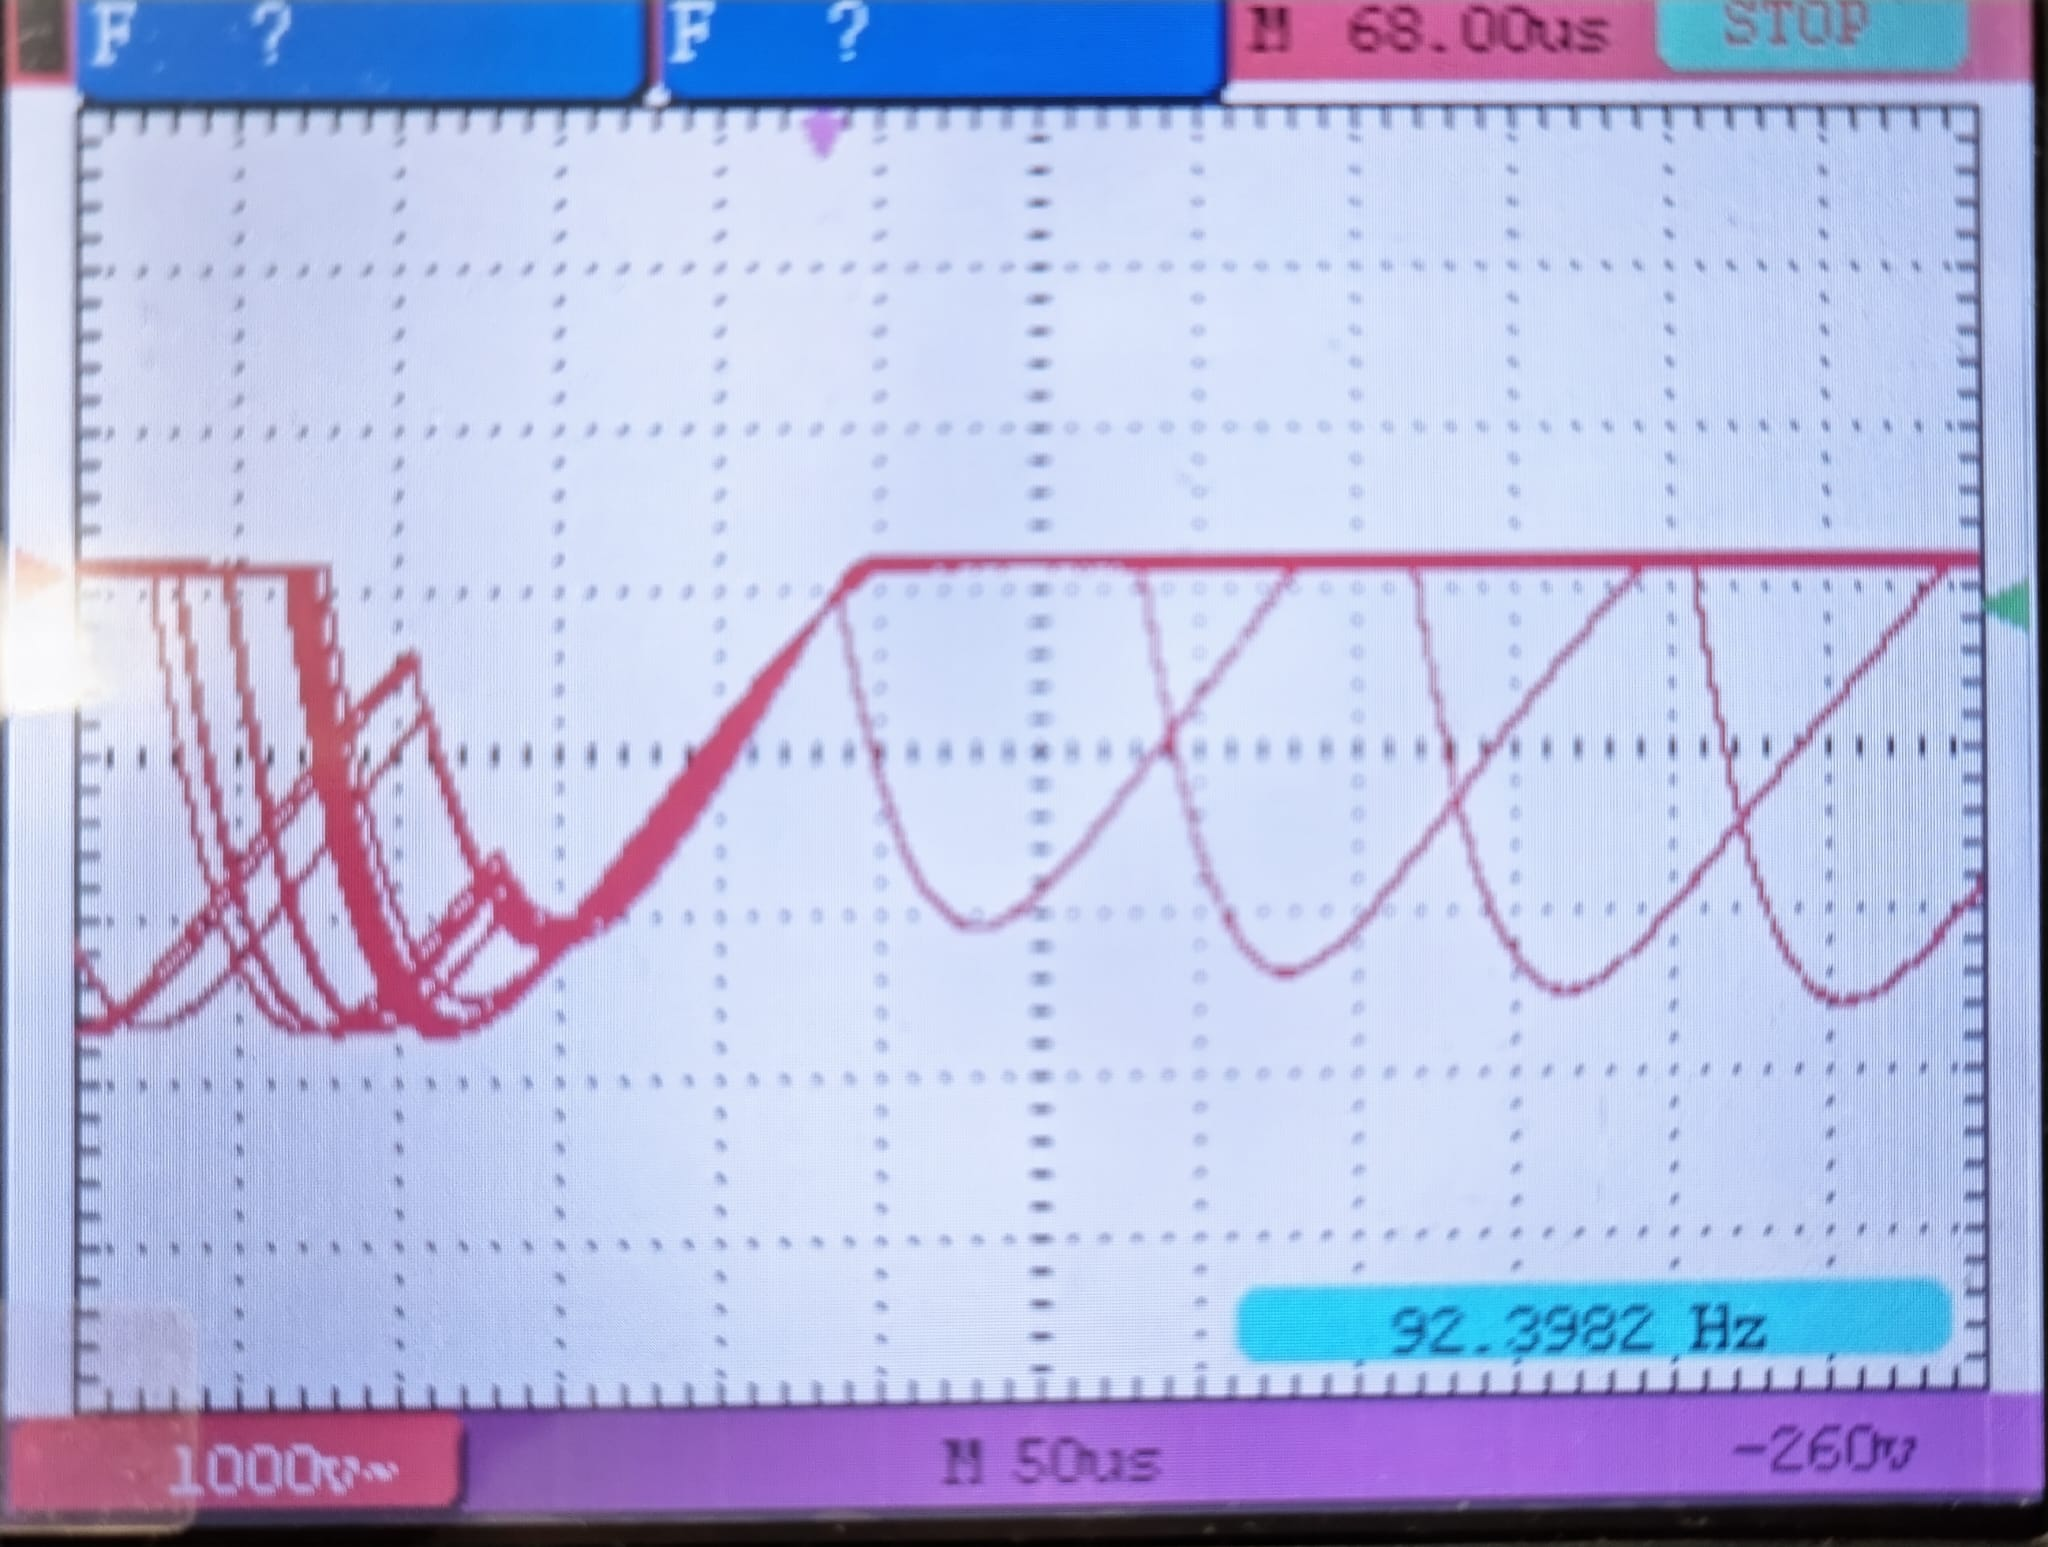
\includegraphics[width = \textwidth]{content/totzeit.jpg}
  \caption{Oszillogramm zur Bestimmung der Totzeit des Geiger-Müller-Zählrohres.}
  \label{fig:totzeit}
\end{figure}
Die Nachentladungszeit lässt sich aus dem Abstand zwischen des Maximums des ersten Peaks bis zum Maximum des zweiten Peaks ablesen. Es kann die Zeit
\begin{equation*}
  T_n=3.6\cdot 50\ \mu s=180\ \mu s
\end{equation*}
abgelesen werden. 

\subsubsection{Zwei-Quellen-Methode}
 Für die Zwei-Quellen-Methode ergeben sich die Messwerte unter Einbezug des 
 Poisson-Fehlers und der Integrationszeit von $120$s zu $N1 = \frac{21844 \pm 148}{120s}$, $N2 = \frac{17594 \pm 133}{120s}$ 
 und $N12 = \frac{39105 \pm 198}{120s}$.
 Es wird für den Strom $I$ eine Ableseungenauigkeit von $\Delta I = 0,05 \mu$A angenommen, für die Zählrate 
 gilt das Vertrauensintervall $\pm \frac{\sqrt{N}}{t}$.\\
 Mit \autoref{eq:2} berechnet sich die Totzeit zu $T_2 = 50 \pm 40 \mu \;$s.
Der Fehler nach Gauß ergibt sich hier durch 
\begin{equation*}
\Delta T = \sqrt{(- \frac{1}{2 N_1^2 N_2})^2(\Delta N_1)^2+(- \frac{1}{2 N_2^2 N_1})^2(\Delta N_2)^2+(- \frac{1}{2 N_1 N_2})^2(\Delta N_{12})^2}
\end{equation*}

\subsection{Freigesetzte Ladungsmenge}

Die freigesetze Ladungsmenge wird nach \autoref{eq:5} aus dem Zählrohrstrom
bestimmt.\\
Der Fehler dieser Formel lässt sich aus % Delta Z = ( (∂z/∂i)^2 * ∆i^2 +  (∂z/∂n)^2 * ∆n^2 )^1/2
\begin{equation*}
  \Delta Z = \sqrt{ ( \frac{1}{e_0 \cdot N} )^2 \cdot (\Delta I)^2 + (- \frac{I}{e_0 \cdot N^2})^2 \cdot (\Delta N)^2}
\end{equation*}
bestimmen.
Sie ist in Abhängigkeit vom Strom in \autoref{fig:lad} graphisch dargestellt.\\
\begin{figure}[H]
  \centering
  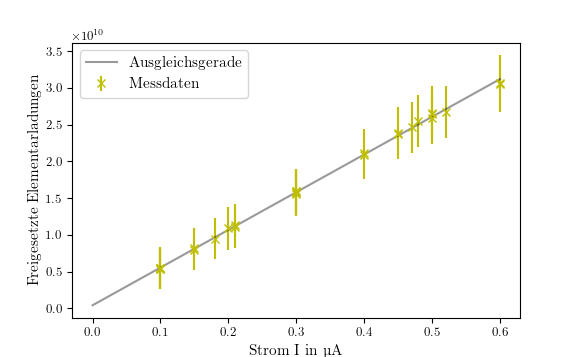
\includegraphics[width=12cm]{content/hobelneu.png}
  \caption{Die freigesetze Ladungsmenge je einfallendem Teilchen in Abhängigkeit vom Strom.}
  \label{fig:lad}
\end{figure}

